\section{Prospetto economico}
Vengono mostrati i prospetti economici per ciascun periodo di progetto, divisi per ruolo. I periodi di \AR{} e \AD{} non sono a carico del Committente.

\subsection{\AR}
Nel periodo di \AR{} le ore sono suddivise nel modo seguente:
\begin{table}[H]
	\centering
	\begin{tabular}{|c|c|c|}
		\hline
		\textbf{Ruolo} &
		\textbf{Ore} &
		\textbf{Costo} \\
		\hline
		Responsabile & 30 & 900\\
		\hline
		Amministratore & 29 & 580\\
		\hline
		Analista & 90 & 2250\\
		\hline
		Progettista & 0 & 0 \\
		\hline
		Programmatore & 0 & 0 \\
		\hline
		Verificatore & 40 & 600\\
		\hline
		\textbf{Totale} & \textbf{189} & \textbf{4330} \\
		\hline
	\end{tabular}
	\caption{Costo per ruolo, periodo di \AR}
\end{table}

I seguenti grafici mostrano visivamente come influiranno i ruoli per ore e costi nel periodo di \AR.
\begin{figure}[H]
	\centering
	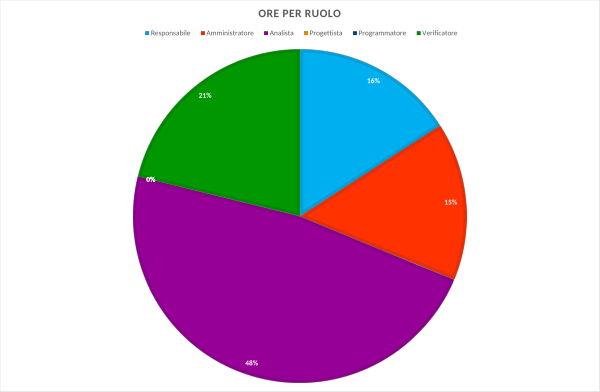
\includegraphics[width=14cm]{img_peconomico/AA_OR.png}
	\caption{Ore per ruolo, periodo di \AR}
\end{figure}
\begin{figure}[H]
	\centering
	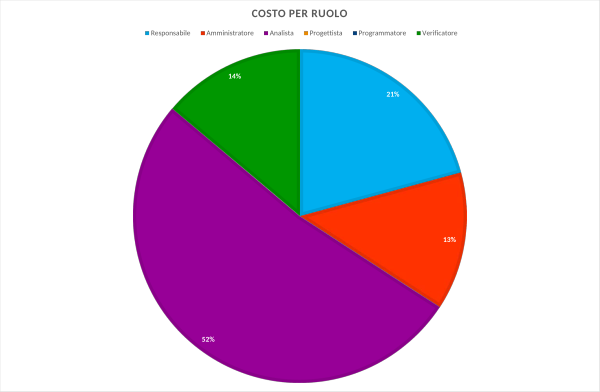
\includegraphics[width=14cm]{img_peconomico/AA_CR.png}
	\caption{Costi per ruolo, periodo di \AR}
\end{figure}

\subsection{\AD}
Nel periodo di \AD{} le ore sono suddivise nel modo seguente:
\begin{table}[H]
	\centering
	\begin{tabular}{|c|c|c|}
		\hline
		\textbf{Ruolo} &
		\textbf{Ore} &
		\textbf{Costo} \\
		\hline
		Responsabile & 1 & 30\\
		\hline
		Amministratore & 1 & 20\\
		\hline
		Analista & 15 & 375\\
		\hline
		Progettista & 0 & 0 \\
		\hline
		Programmatore & 0 & 0 \\
		\hline
		Verificatore & 4 & 60\\
		\hline
		\textbf{Totale} & \textbf{21} & \textbf{485} \\
		\hline
	\end{tabular}
	\caption{Costo per ruolo, periodo di \AD}
\end{table}

I seguenti grafici mostrano visivamente come influiranno i ruoli per ore e costi nel periodo di \AD.
\begin{figure}[H]
	\centering
	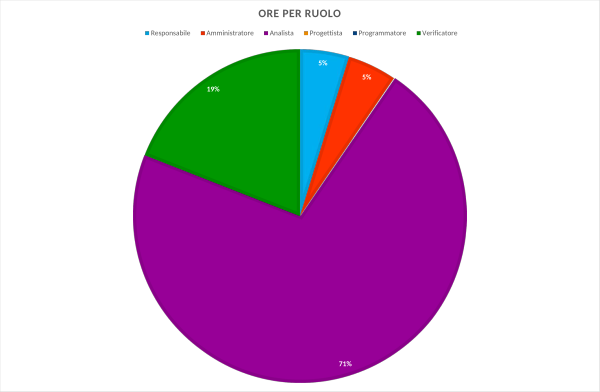
\includegraphics[width=14cm]{img_peconomico/AD_OR.png}
	\caption{Ore per ruolo, periodo di \AD}
\end{figure}
\begin{figure}[H]
	\centering
	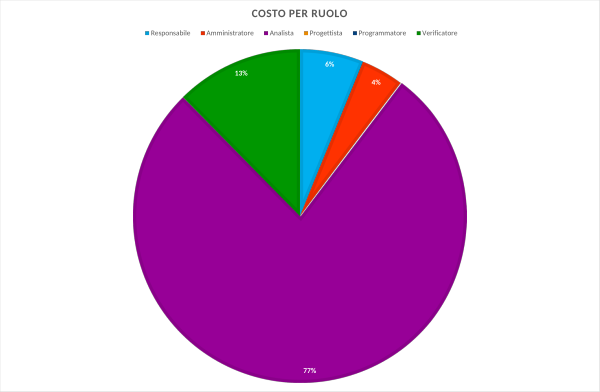
\includegraphics[width=14cm]{img_peconomico/AD_CR.png}
	\caption{Costi per ruolo, periodo di \AD}
\end{figure}

\subsection{\PA}
Nel periodo di \PA{} le ore sono suddivise nel modo seguente:
\begin{table}[H]
	\centering
	\begin{tabular}{|c|c|c|}
		\hline
		\textbf{Ruolo} &
		\textbf{Ore} &
		\textbf{Costo} \\
		\hline
		Responsabile & 8 & 240\\
		\hline
		Amministratore & 6 & 120\\
		\hline
		Analista & 23 & 575\\
		\hline
		Progettista & 101 & 2222 \\
		\hline
		Programmatore & 0 & 0 \\
		\hline
		Verificatore & 55 & 825\\
		\hline
		\textbf{Totale} & \textbf{193} & \textbf{3982} \\
		\hline
	\end{tabular}
	\caption{Costo per ruolo, periodo di \PA}
\end{table}

I seguenti grafici mostrano visivamente come influiranno i ruoli per ore e costi nel periodo di \PA.
\begin{figure}[H]
	\centering
	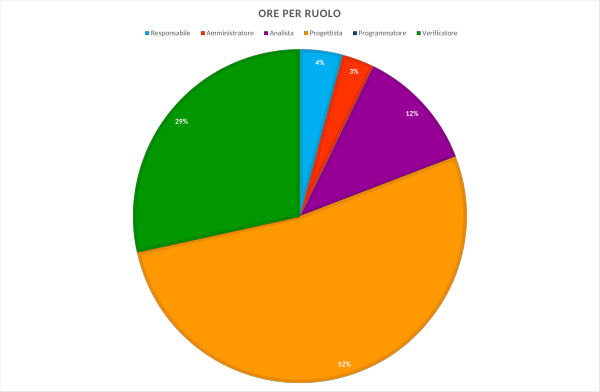
\includegraphics[width=14cm]{img_peconomico/PA_OR.png}
	\caption{Ore per ruolo, periodo di \PA}
\end{figure}
\begin{figure}[H]
	\centering
	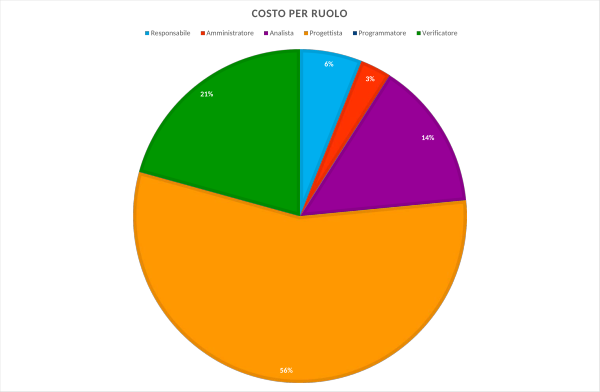
\includegraphics[width=14cm]{img_peconomico/PA_CR.png}
	\caption{Costi per ruolo, periodo di \PA}
\end{figure}

\subsection{\PD}
Nel periodo di \PD{} le ore sono suddivise nel modo seguente:
\begin{table}[H]
	\centering
	\begin{tabular}{|c|c|c|}
		\hline
		\textbf{Ruolo} &
		\textbf{Ore} &
		\textbf{Costo} \\
		\hline
		Responsabile & 8 & 240 \\
		\hline
		Amministratore & 8 & 160 \\
		\hline
		Analista & 4 & 100\\
		\hline
		Progettista & 107 & 2354 \\
		\hline
		Programmatore & 0 & 0 \\
		\hline
		Verificatore & 36 & 540 \\
		\hline
		\textbf{Totale} & \textbf{163} & \textbf{3394} \\
		\hline
	\end{tabular}
	\caption{Costo per ruolo, periodo di \PD}
\end{table}

I seguenti grafici mostrano visivamente come influiranno i ruoli per ore e costi nel periodo di \PD{}.
\begin{figure}[H]
	\centering
	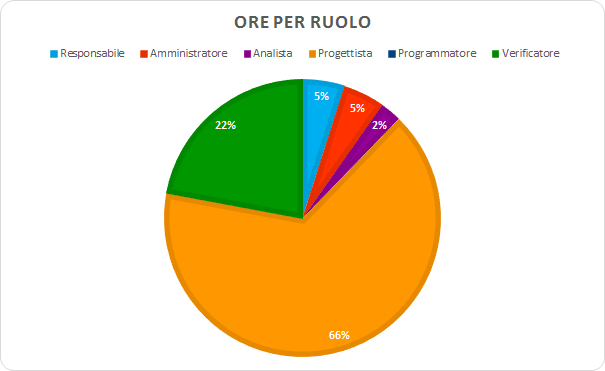
\includegraphics[width=14cm]{img_peconomico/PD2_OR.png}
	\caption{Ore per ruolo, periodo di \PD}
\end{figure}
\begin{figure}[H]
	\centering
	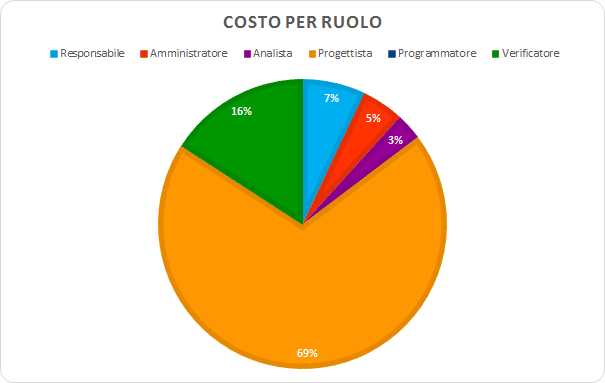
\includegraphics[width=14cm]{img_peconomico/PD2_CR.png}
	\caption{Costi per ruolo, periodo di \PD}
\end{figure}

\subsection{\Cod}
Nel periodo di \Cod{} le ore sono suddivise nel modo seguente:
\begin{table}[H]
	\centering
	\begin{tabular}{|c|c|c|}
		\hline
		\textbf{Ruolo} &
		\textbf{Ore} &
		\textbf{Costo} \\
		\hline
		Responsabile & 9 & 270 \\
		\hline
		Amministratore & 4 & 80 \\
		\hline
		Analista & 0 & 0\\
		\hline
		Progettista & 16 & 352 \\
		\hline
		Programmatore & 147 & 2205 \\
		\hline
		Verificatore & 55 & 825 \\
		\hline
		\textbf{Totale} & \textbf{231} & \textbf{3732} \\
		\hline
	\end{tabular}
	\caption{Costo per ruolo, periodo di \Cod}
\end{table}

I seguenti grafici mostrano visivamente come influiranno i ruoli per ore e costi nel periodo di \Cod.
\begin{figure}[H]
	\centering
	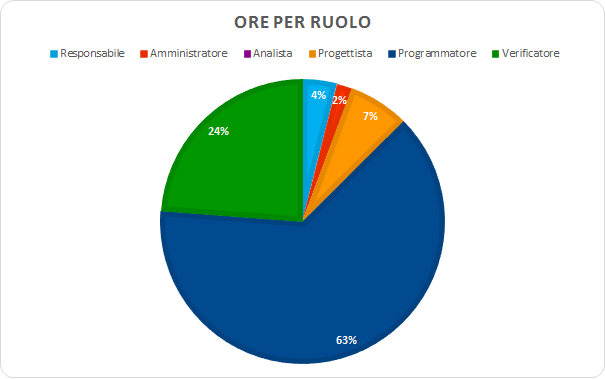
\includegraphics[width=14cm]{img_peconomico/C2_OR.png}
	\caption{Ore per ruolo, periodo di \Cod}
\end{figure}
\begin{figure}[H]
	\centering
	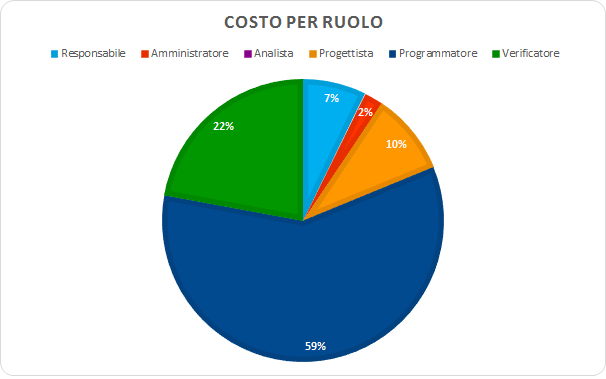
\includegraphics[width=14cm]{img_peconomico/C2_CR.png}
	\caption{Costi per ruolo, periodo di \Cod}
\end{figure}

\subsection{\VV}
Nel periodo di \VV{} le ore sono suddivise nel modo seguente:
\begin{table}[H]
	\centering
	\begin{tabular}{|c|c|c|}
		\hline
		\textbf{Ruolo} &
		\textbf{Ore} &
		\textbf{Costo} \\
		\hline
		Responsabile & 10 & 300\\
		\hline
		Amministratore & 16 & 320\\
		\hline
		Analista & 0 & 0\\
		\hline
		Progettista & 13 & 286 \\
		\hline
		Programmatore & 12 & 180 \\
		\hline
		Verificatore & 83 & 1245\\
		\hline
		\textbf{Totale} & \textbf{134} & \textbf{2331} \\
		\hline
	\end{tabular}
	\caption{Costo per ruolo, periodo di \VV}
\end{table}

I seguenti grafici mostrano visivamente come influiranno i ruoli per ore e costi nel periodo di \VV{}.
\begin{figure}[H]
	\centering
	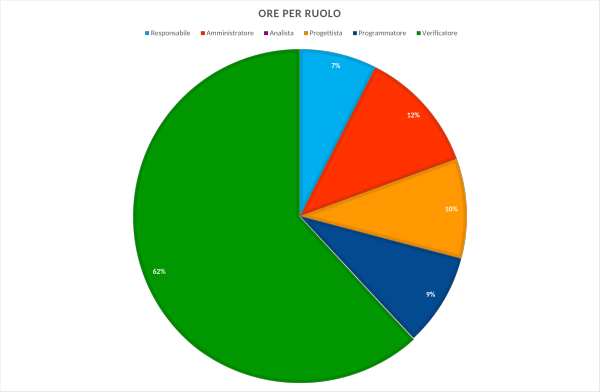
\includegraphics[width=14cm]{img_peconomico/VV_OR.png}
	\caption{Ore per ruolo, periodo di \VV}
\end{figure}
\begin{figure}[H]
	\centering
	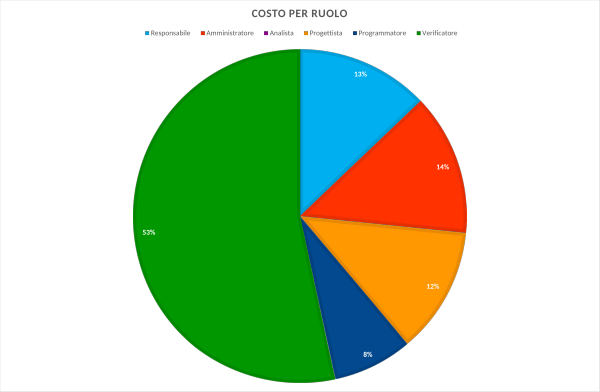
\includegraphics[width=14cm]{img_peconomico/VV_CR.png}
	\caption{Costi per ruolo, periodo di \VV}
\end{figure}

\subsection{Totale}
\subsubsection{Ore totali con investimento}
Le ore complessive previste per ogni ruolo sono riportate nella tabella sottostante.
\begin{table}[H]
	\centering
	\begin{tabular}{|c|c|c|}
		\hline
		\textbf{Ruolo} &
		\textbf{Ore} &
		\textbf{Costo} \\
		\hline
		Responsabile & 66 & 1980\\
		\hline
		Amministratore & 64 & 1280\\
		\hline
		Analista & 132 & 3300\\
		\hline
		Progettista & 237 & 5214 \\
		\hline
		Programmatore & 159 & 2385 \\
		\hline
		Verificatore & 273 & 4095\\
		\hline
		\textbf{Totale} & \textbf{931} & \textbf{18254} \\
		\hline
	\end{tabular}
	\caption{Costo totale per ruolo}
\end{table}
I seguenti grafici mostrano visivamente come influiranno i ruoli per ore e costi nel progetto.
\begin{figure}[H]
	\centering
	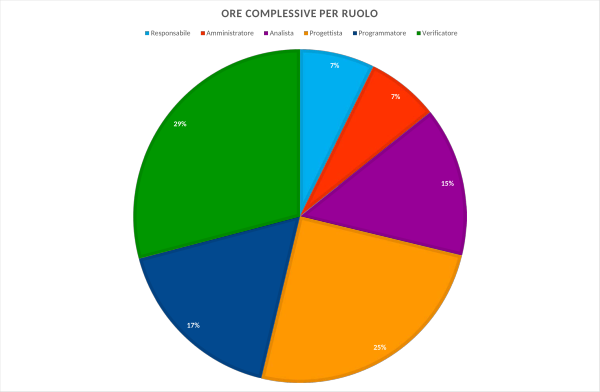
\includegraphics[width=14cm]{img_peconomico/T_OR_C.png}
	\caption{Ore totali per ruolo}
\end{figure}
\begin{figure}[H]
	\centering
	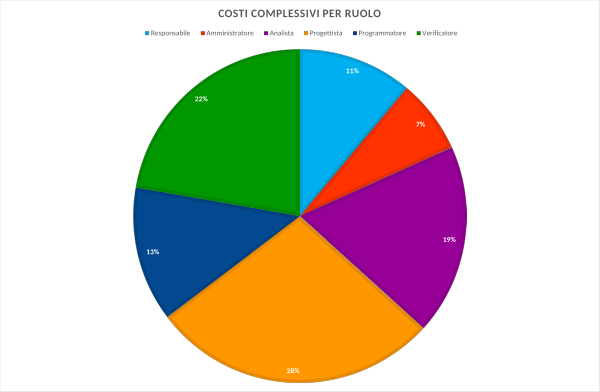
\includegraphics[width=14cm]{img_peconomico/T_CR_C.png}
	\caption{Costi totali per ruolo}
\end{figure}

\subsubsection{Ore totali senza investimento}
Le ore complessive rendicontate per ogni ruolo, cioè quelle senza investimento iniziale, sono riportate nella tabella sottostante.
\begin{table}[H]
	\centering
	\begin{tabular}{|c|c|c|}
		\hline
		\textbf{Ruolo} &
		\textbf{Ore} &
		\textbf{Costo} \\
		\hline
		Responsabile & 35 & 1050\\
		\hline
		Amministratore & 34 & 680\\
		\hline
		Analista & 27 & 675\\
		\hline
		Progettista & 237 & 5214 \\
		\hline
		Programmatore & 159 & 2385 \\
		\hline
		Verificatore & 229 & 3435\\
		\hline
		\textbf{Totale} & \textbf{721} & \textbf{13439} \\
		\hline
	\end{tabular}
	\caption{Costo totale senza investimento per ruolo}
\end{table}
I seguenti grafici mostrano visivamente come influiranno i ruoli per ore e costi nel progetto.
\begin{figure}[H]
	\centering
	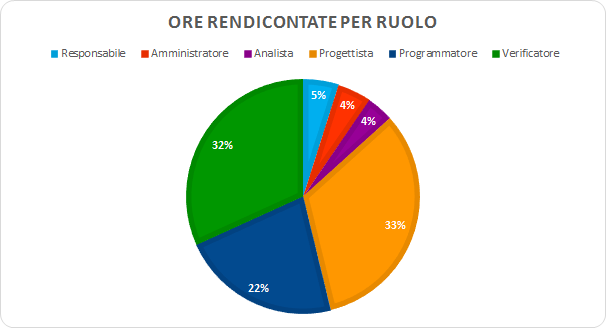
\includegraphics[width=14cm]{img_peconomico/TOT2_OR_R.png}
	\caption{Ore totali senza investimento per ruolo}
\end{figure}
\begin{figure}[H]
	\centering
	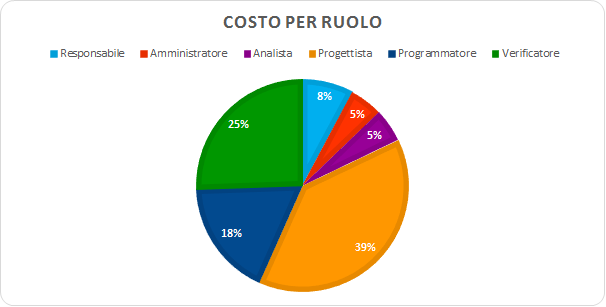
\includegraphics[width=14cm]{img_peconomico/TOT2_CR_R.png}
	\caption{Costi totali senza investimento per ruolo}
\end{figure}





